% This is not a step-by-step instruction or diary to your work.
% Instead, you should describe your technical approach and solution, describe architecture, components, etc.
% Think software engineering...
% Perhaps use a few useful uml-diagrams or illustrate the system architecture.
% Keep in mind that the purpose of the implementation section is to describe your implementation to solve the problems from 1.3.
 
% This section can have a lot of subsections, example:
% 4.1 System architecture / System arkitektur
% 4.2 System components / System komponenter
% 4.3 ...

% TODO: Explain design methods used. Modulare, Singelthon and so on.

Three projects comprise the implementation, the first being a debug library named \emph{rust-debug}.
Its purpose is to simplify retrieving debug information from the \gls{DWARF} format.
The second project is the debugger \gls{erdb} which implements the \gls{dap} protocol.
The last project is a \emph{VSCode} extension that launches the \gls{erdb} debugger and connects to it.


\section{Debugging Library \emph{rust-debug}}
\label{section:rust-debug}
Retrieving debug information from the \gls{DWARF} sections in the \gls{elf} file is one of the main problems that must be solved when creating a debugger.
The \emph{Rust} library \emph{gimli-rs} simplifies that problem by providing data structures and functions for reading the \gls{DWARF} sections.
However, the library requires the user to know the \gls{DWARF} format, the target system, and the programming language/compiler.
The \emph{rust-debug} library is created to make it possible to get information from the \gls{DWARF} format for someone without that knowledge.


Some of the main functionality that \emph{rust-debug} provides solutions for are the following:

\begin{itemize}
  \item Retrieve the source code file location where functions, variables, types, and more are declared.
  \item Virtually unwinding the call stack.
  \item Evaluating variables.
  \item Translating source file line number to the nearest machine code address.
  \item Finding the \gls{die} that represents a function using the name.
\end{itemize}

The code for this library is in the \emph{GitHub} repository \cite{rust-debug}.



\subsection{Retrieving Source Code File Location} \label{sec:decl}
In the \gls{DWARF} format, the source code location where any data was declared is stored in three attributes on the \gls{die} representing that data.
One attribute contains indirect information about which file the data was declared, another contains the line number, and the last contains the column number.


The attribute contains the file path and name information named \emph{DW\_AT\_decl\_file}.
It does not contain the file path and name directly.
Instead, it contains a file index.
This file index is used to look up the file path and name in a line number information table, and each compilation unit has one such table.
File index 0 is reserved and used when the source file is unknown.


The source code line and column number can be read directly from the attributes \emph{DW\_AT\_decl\_line} and \emph{DW\_AT\_decl\_column}, respectively.
Thus, they are much easier to retrieve.


\emph{Rust-debug} provides a function that performs the file index lookup and gets the line and column numbers.
The function requires that a DIE and related compilation unit is given.


\subsection{Accessing Memory And Registers}
Some functionalities in the \gls{DWARF} format require access to register and memory.
One of them is the evaluation of variables.


Accessing the debug target registers and memory is a different problem from reading and using the \gls{DWARF} format.
Thus, \emph{rust-debug} lets the user of the library solve that problem.
It has the benefit that any existing solutions can be used, like \emph{probe-rs}.
It also has one downside, \emph{rust-debug} is harder to use because of the extra work the user must do.


All the functionalities in \emph{rust-debug} that require access to the registers require a struct named \emph{Registers}.
This struct contains a \emph{HashMap} with the register numbers and their corresponding values, and it also contains the register number of some special registers, like the \gls{pc} register.
Therefore, it is up to the user to fill in the correct register numbers and values.
An example of implementing this can be found in the git repository for \gls{erdb} \cite{erdb}.


The functionalities that require access to the debug target's memory require a struct that implements the \emph{rust-debug} trait \emph{MemoryAccess}.
This trait is straightforward and only has one function: reading various bytes at a given address.
Users can create a struct that implements that function almost however they want.
An example of implementing this using the \emph{probe-rs} library can be found in the git repository for \gls{erdb} \cite{erdb}.



\subsection{Evaluating Variables} \label{sec:ievalvar}
To make evaluating a variable's value and retrieving other information about the variable easy, \emph{rust-debug} provides a struct named \emph{Variable}.
That struct only has one function named \emph{get\_variable}, which takes a \gls{die} and returns a \emph{rust-debug} \emph{Variable} struct.
The \emph{rust-debug} \emph{Variable} struct may contain the following information:


\begin{itemize}
  \item Variable name.
  \item Variable value, type, and location on the debug target. All this information is stored in a tree structure.
  \item Variable declaration location, the file, line, and column.
\end{itemize}


All the information in the Variable struct may not be present because not all \glspl{die} contain the information the struct may have.


The evaluated value of a variable is represented in a tree structure.
The structure is similar to how the information is stored in the \gls{DWARF} format.
However, the value of each branch is evaluated into a primary value type, such as a signed integer.
Therefore, it removes the most challenging part of evaluating a variable without losing the flexibility of the \gls{DWARF} format.
The only downside of this solution is that it requires the user to understand how variables are structured in the \gls{DWARF} format.


\subsection{Finding the current function} \label{sec:funcdie}
When debugging, knowing the current function that is being executed is very useful.
Finding that function can be done by finding the function \gls{die}, which is the furthest down the \gls{die} tree, in the branch where the current address is in range.
Thus, the function \gls{die} can easily be found by tracking all the function \glspl{die} while going down the \gls{die} tree.
\emph{Rust-debug} makes this even easier by providing a function that does exactly this.



\subsection{Unwinding the Call Stack}
The \emph{rust-debug} library has a function for virtually unwinding the current call stack, and it does it in two separate steps.
Unwinding the call stack to get all the register values for each stack frame is the first step.
The second step is to find the subroutine and evaluate all the variables for each stack frame.


Unwinding the call stack to get the register values is done by a separate function, which returns a \emph{Vec} of \emph{CallFrame} structs.
Each \emph{CallFrame} struct contains information about each of the stack frames.
The essential information the struct contains is the unwound register values, but it also contains other helpful information, such as the stack frame's start and end memory addresses.
All the information in the struct is retrieved using the method described in section \ref{sec:stacktrace}.


In the second step, the function loops through all the \emph{CallFrame} structs and tries to retrieve all the information it can about the stack frame.
It includes the subroutine's name and the declaration location, which is found using the function described in section \ref{sec:decl}.
It also includes the variable information retrieved using the function described in section \ref{sec:ievalvar}.



\subsection{Finding Breakpoint Location}
The \emph{rust-debug} library has a function that finds a machine code address using a source code location.
This machine code location is the closest one that represents the given line in the source code.
The function requires a file path and line number, but it also can take a column number.


The mentioned function works by first finding out which compilation unit contains information on the inputted file path.
It does this by looping through all the file entries in the line number information table for every compilation unit.
Each line number information table entry has rows containing information on a line from the source code.
All the rows with the search line numbers are added to a list.
The machine code address of the first element in this list is returned if no column line was inputted into the function.
Otherwise, the one with the closest column number is returned.



\section{Embedded Rust Debugger}
The \acrfull{erdb} is implemented using the debugging library \emph{rust-debug}, which requires the \emph{gimli-rs} library.
\emph{Rust-debug} provides all the needed functionalities for retrieving debug information from the \gls{DWARF} format.
The debugger also uses the \emph{probe-rs} library for controlling the debug target, and it is also used for accessing the registers and memory of the debug target.


The debugger consists of three modules.
The first one is named \acrshort{cli}.
Its primary function is to handle the input and output from the terminal.
The second module is named \emph{DebugAdapter}.
It also handles the input and output, but in the form of \gls{dap} messages.
These \gls{dap} messages are sent through a \acrshort{tcp} connection and are for supporting the \gls{dap} protocol.
The last module is named \emph{Debugger}.
It is for getting debug information and controlling the debug target.


The debugger is implemented asynchronously because all the modules handle input from the user or the debug target.
Therefore, the main loop waits for input from any modules and then handles them.
Figure \ref{fig:ERDStruct} shows a diagram of how these modules are structured.


\begin{figure}[h]
	\centering
	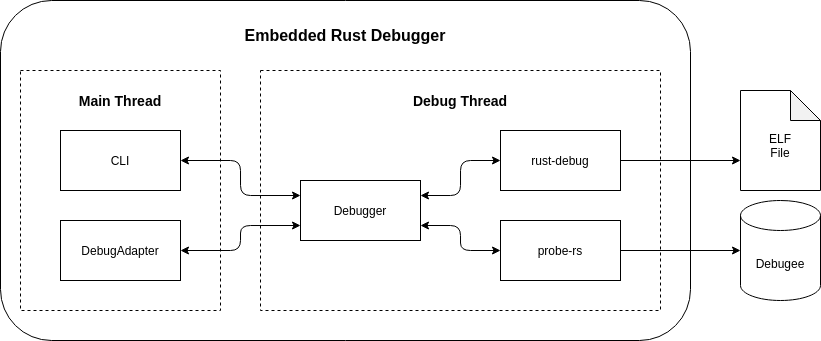
\includegraphics[width=1.0\textwidth]{debugger_structure.png}
	\caption{Diagram showing the structure of \gls{erdb}.}
	\label{fig:ERDStruct}
\end{figure}


The code for \gls{erdb} can be found in this git repository \cite{erdb}.


\subsection{The CLI Module} 
The \acrshort{cli} module has two jobs.
The first is to read and parse the input from the terminal into a request that the \emph{Debugger} module can understand.
The second is to convert the responses from the Debugger module to text and output that text to the terminal.


Reading the input from the terminal is done asynchronously, which enables other tasks to be done while the \acrshort{cli} waits for the user input.
When a new line has been entered, the \acrshort{cli} module will try to parse the string into a \emph{DebugRequest} enum.
The string is parsed by matching the first word in the string to a command.
Also, each command has a parser that is then used to parse the rest of the string.
The resulting \emph{DebugRequest} enum is then returned to the main loop and sent to the \emph{Debugger} module.


After the \emph{Debugger} module has done its work, the result is printed to the terminal.
It is done by sending the \emph{DebugResponse} enum that the \emph{Debugger} module returned to a function that has a match for each of the enum variants.
Each variant has a unique message printed to the terminal, and the messages often contain data from the \emph{DebugResponse} enum.
A helpful message is printed to the terminal if the input text cannot be parsed.


There is also a \emph{DebugEvent} enum, that is printed to the terminal in the same way the \emph{DebugResponse} is.
The \emph{DebugEvent} enum is created by another task, which polls the debug target state.
That task's primary job is to report if the debug target has halted the program that is being debugged.



\subsection{The Debug Adapter module}
All the \gls{dap} communication is handled in the \emph{debug adapter} module.
The main job of this module is to translate \gls{dap} messages into requests, which are forwarded to the \emph{debugger} module.
It also handles the translation of the responses and events from the \emph{debugger} module.


The DAP protocol communicates through \gls{tcp}, requiring the \emph{debug adapter} module to have a \gls{tcp} server.
All the \gls{tcp} communication is handled asynchronously, and it is to enable the other tasks to run simultaneously.
Currently, only one \gls{tcp} connection can be open at a time, and it is because the rest of the system still needs to support multiple simultaneous debugging sessions.



\subsection{The Debugger Module}
The \emph{debugger} module primarily consists of one struct named \emph{DebugHandler}.
Its primary job is to get the debug information from the \gls{DWARF} format, and another is to keep track of the debug targets state.
This struct only has two methods for accomplishing its jobs, one for polling the state of the debug target.
The other method, named \emph{handle\_request}, takes a \emph{DebugRequest} as an argument and calls a function based on the argument.
The method also returns a \emph{DebugResponse} with the result.


The general flow when the \emph{handle\_request} method is called is as follows.


First, the \emph{DebugRequest} enum is matched, and a check is done to see that all the required information is present.
Then, the \emph{debugger} module will perform some task related to the given argument, which often involves using the \emph{probe-rs} library to access the debug target and/or the rust-debug for retrieving debug information.
Lastly, the result is returned using the enum \emph{DebugResponse}.



\subsubsection{Retrieving Debug Information}
The \emph{debugger} module retrieves debug information by using the \emph{rust-debug} library.
That library sometimes requires values from the debug target, such as the values stored in registers and memory addresses, and those values are retrieved from the debug target using \emph{probe-rs}.



\subsubsection{Simultaneous Handling of Requests And Events}
% How the debugger handles request and events simultaneously.
The state of the debug target is polled every $100\text{th}$ millisecond, to detect if the debug target has continued or stopped the program execution.
In the time between the polls other tasks can be handled, such as parsing the input from the \acrshort{cli} or doing a stack trace.
This is possible because there is an asynchronous function which sleeps for $100$ milliseconds, afterwards it polls the debug target state.
That function repeats if the debug target is being debugged.
Thus, the debugger can simultaneously handle both input from the user and state changes in the debug target.
A state change in the debug target is referred to as an event in \gls{erdb}.



\subsubsection{Optimization of Repeated Variable Evaluation}
% How it handles request for stackframes and variables.
To improve on the performance of the debugger, all the variables and stack frames are temporarily stored.
This allows for fast repetitive lookup of debug information.
All this temporarily stored information is removed when the state of the debug target changes.
This is to ensure that the correct information is returned.


Note that if a request is received to evaluate one variable, the debugger will then perform a whole stack trace instead.
This simplifies the implementation a lot, it also makes the subsequent evaluation requests faster.
Because, the value does not need to be evaluated, instead it can be taken from temporarily stored information.



\section{VSCode Extension}
% Explain the implementation of the vscode explanation.
Creating a \emph{VSCode} extension is simple because \emph{Microsoft} has a tool named \emph{vscode-generator-code} \cite{vscode-generator-code}, that will generate a empty extension.
The provided documentations also explain how to get started with creating an extension.


There are two different types of debug extensions, the first is an extension that implements a debug adapter for a specific debugger.
These often require a lot of work because a debug adapter needs to translate the \gls{dap} protocol messages to command that the debugger understands.
Depending on the debugger this can require a lot of work to get it working well.
The other type of debug extension is just a wrapper for the debugger that already implements the \gls{dap} protocol.
These extensions are very simple to create, because they only need to start the debugger and connect to it using the \emph{dap} protocol.
To learn more about \emph{VSCode} debug extension read \emph{Microsofts} documentations \cite{vscode-debugger-extension-doc}.


The debugger \emph{Embedded Rust Debugger} implements the \gls{dap} protocol over a \gls{tcp} server.
The \emph{VSCode} extension is just a wrapper that starts the debugger \gls{tcp} server and then connects to it.
Connecting to the debugger server over \gls{tcp} is very easy to do because \emph{Microsoft} has a library named \emph{VSCode} that does that for you.
The extension also captures the logs of the debugger and outputs them to the user using the \emph{VSCode} library.


There are also some configurations that the user of the \gls{erdb} can set in the \emph{launch.json} file.
The available configurations are defined in a \emph{json} file named \emph{package.json} in the extension project \cite{erdb-vscode}.
